%%%%%%Experiments%%%%%%%%
\section{Experiments}\label{sec:experiments}
In this section, we empirically demonstrate the effectiveness of the proposed distributional matching framework in visual tokenization tasks.
Experiments are conducted within the VQ-VAE~\cite{Oord2017NeuralDR} and VQGAN~\cite{Esser2020TamingTF} frameworks. %PyTorch code, including training scripts and logs, will be made publicly available.

\subsection{Evaluation on VQ-VAE Framework}
\label{sec:vqvae experiments}
\paragraph{Datasets and Baselines} Experiments are conducted on four benchmark datasets: two low-resolution datasets, i.e., CIFAR-10~\cite{Krizhevsky2009LearningML} and SVHN~\cite{Netzer2011ReadingDI},  and two high-resolution datasets FFHQ~\cite{Karras2018ASG} and ImageNet~\cite{Deng2009ImageNetAL}. We evaluate our approach against representative VQ methods:  Vanilla VQ~\cite{Oord2017NeuralDR}, EMA VQ~\cite{Razavi2019GeneratingDH}, which uses exponential moving average updates and is also referred to as $k$-means, Online VQ, which employs $k$-means++ in CVQ-VAE~\cite{Zheng2023OnlineCC}, and enhanced  straight-through estimator STE++~\cite{Huh2023StraighteningOT}. For experimental settings, see Appendix~\ref{appendix:experimental details}. 

\paragraph{Metrics}
We employ multiple evaluation metrics, including the codebook utilization rate ($\mathcal{U}$), codebook perplexity ($\mathcal{C}$), peak signal-to-noise ratio (PSNR), patch-level structural similarity index (SSIM), and pixel-level reconstruction loss (Rec. Loss).
We exclude the raw quantization error ($\mathcal{E}$) from the main VQ-VAE experiments, as $\mathcal{E}$ is highly sensitive to feature variance, which is not controlled under different training dynamics. Consequently, a direct comparison of $\mathcal{E}$ does not faithfully reflect the intrinsic effectiveness of VQ algorithms, as discussed in Section~\ref{sec:distributional formulation} and Section~\ref{sec:atomic setting}.

%from the main results. 
%As analyzed in Appendix~\ref{appendix:Impact of Distribution Variance}, $\mathcal{E}$ is highly sensitive to the scale of feature variance, which varies across different methods. 
%Consequently, a direct comparison of $\mathcal{E}$ without controlling for variance is potentially misleading. 
%To ensure a rigorous assessment, we provide a controlled ``atomic setting'' in Appendix~\ref{appendix:discussion}, where distribution variances are strictly normalized to evaluate $\mathcal{E}$ fairly.

\begin{table*}[!t]
  \centering
  \vspace{-1ex}
  \caption{Comparison of VQ-VAEs trained on FFHQ dataset following~\cite{Oord2017NeuralDR}.}
  \label{tab:vqvae ffhq}
  \vspace{-1ex}
  \resizebox{0.9\textwidth}{!}{%
  \begin{tabular}{@{}lccccccc@{}} \hline
    Approaches & Tokens & Codebook Size & $\mathcal{U}$ ({\color{green!60!black}\bfseries$\pmb{\uparrow}$}) & $\mathcal{C}$ ({\color{green!60!black}\bfseries$\pmb{\uparrow}$}) & PSNR({\color{green!60!black}\bfseries$\pmb{\uparrow}$}) & SSIM({\color{green!60!black}\bfseries$\pmb{\uparrow}$}) & Rec. Loss({\color{green!60!black}\bfseries$\pmb{\downarrow}$}) \\\hline
    Vanilla VQ  & 256 & $16384$ & 3.8\% & 527.2 & 27.83 & 73.8 & 0.0119 \\ 				
    STE++ & 256 & $16384$ & 3.4\% & 476.7 & 27.54 & 72.3 & 0.0129 \\
    EMA VQ & 256 & $16384$ & 14.0\% & 1795.7 & 28.39 & 74.8 & 0.0106 \\
    Online VQ  & 256 & $16384$ & 11.7\% & 1115.3 & 27.68 & 72.6 & 0.0125 \\
    \textbf{Wasserstein VQ} & 256 & $16384$ & \textbf{100\%} &  \textbf{15713.3} & \textbf{29.03} & \textbf{76.6} & \textbf{0.0093} \\\hline
    Vanilla VQ & 256 & $50000$ & 1.2\% & 516.8 & 27.83 & 73.6 & 0.0120  \\ 				
    STE++ & 256 & $50000$ & 1.0\% & 447.2 & 27.49 & 72.4 & 0.0131\\
    EMA VQ & 256 & $50000$ & 10.3\% & 4075.7 & 28.61 & 75.3 & 0.0101 \\
    Online VQ & 256 & $50000$ & 6.0\% & 1642.9 & 28.37 & 74.6 & 0.0107  \\
    \textbf{Wasserstein VQ} & 256 & $50000$ & \textbf{100\%} & \textbf{47496.4} & \textbf{29.24} & \textbf{77.0} & \textbf{0.0089} \\\hline
    Vanilla VQ  & 256 & $100000$ & 0.6\% & 481.0 & 27.86 & 74.2 & 0.0118  \\ 				
    STE++ & 256 & $100000$ & 0.5\% & 450.7 & 27.52 & 72.4 & 0.0130\\
    EMA VQ & 256 & $100000$ & 2.7\% & 2087.5 & 28.43 & 74.8 & 0.0105  \\
    Online VQ & 256 & $100000$ & 3.6\% & 1556.8 & 27.12 & 71.1 & 0.0142 \\
    \textbf{Wasserstein VQ} & 256 & $100000$ & \textbf{100\%} & \textbf{93152.7} & \textbf{29.53} & \textbf{78.0} & \textbf{0.0083} \\\hline
  \end{tabular}
  \vspace{-4ex}
}
\end{table*}

\begin{table*}[!t]
  \centering
  \vspace{-1ex}
  \caption{Comparison of VQ-VAEs trained on ImageNet dataset following~\cite{Oord2017NeuralDR}.}
  \label{tab:vqvae imagenet}
  \vspace{-1ex}
  \small
  \resizebox{0.9\textwidth}{!}{%
  \begin{tabular}{@{}lccccccc@{}}
    \toprule
    \textbf{Methods} & \textbf{Tokens} & \textbf{Codebook Size} & $\mathcal{U}$ ({\color{green!60!black}\bfseries$\pmb{\uparrow}$}) & $\mathcal{C}$ ({\color{green!60!black}\bfseries$\pmb{\uparrow}$}) & \textbf{PSNR} ({\color{green!60!black}\bfseries$\pmb{\uparrow}$}) & \textbf{SSIM} ({\color{green!60!black}\bfseries$\pmb{\uparrow}$}) & \textbf{Rec. Loss} ({\color{green!60!black}\bfseries$\pmb{\downarrow}$}) \\
    \midrule
    Vanilla VQ & 256 & $16{,}384$ & 2.5\% & 360.7 & 24.44 & 57.5 & 0.0294 \\
    STE++ & 256 & $16{,}384$ & 6.5\% & 889.9 & 24.88 & 58.9 & 0.0270 \\
    EMA VQ & 256 & $16{,}384$ & 14.5\% & 1861.5 & 24.98 & 59.2 & 0.0267 \\
    Online VQ & 256 & $16{,}384$ & 22.2\% & 1465.6 & 24.88 & 58.6 & 0.0273 \\
    \textbf{Wasserstein VQ} & 256 & $16{,}384$ & \textbf{100.0\%} & \textbf{15539.1} & \textbf{25.47} & \textbf{61.2} & \textbf{0.0242} \\
    \midrule
    Vanilla VQ  & 256 & $50{,}000$ & 0.9\% & 378.7 & 24.40 & 57.7 & 0.0295 \\
    STE++ & 256 & $50{,}000$ & 2.0\% & 851.7 & 24.89 & 59.0 & 0.0270 \\
    EMA VQ  & 256 & $50{,}000$ & 16.8\% & 6139.3 & 25.37 & 60.9 & 0.0246 \\
    Online VQ & 256 & $50{,}000$ & 9.9\% & 2241.7 & 25.09 & 59.7 & 0.0260 \\
    \textbf{Wasserstein VQ} & 256 & $50{,}000$ & \textbf{100.0\%} & \textbf{46133.2} & \textbf{25.72} & \textbf{62.3} & \textbf{0.0230} \\
    \midrule
    Vanilla VQ & 256 & $100{,}000$ & 0.4\% & 337.0 & 24.43 & 57.4 & 0.0295 \\
    STE++ & 256 & $100{,}000$ & 0.9\% & 730.6 & 24.86 & 59.1 & 0.0269 \\
    EMA VQ  & 256 & $100{,}000$ & 3.0\% & 2170.0 & 25.13 & 60.1 & 0.0257 \\
    Online VQ  & 256 & $100{,}000$ & 4.1\% & 1709.9 & 24.95 & 59.1 & 0.0267 \\
    \textbf{Wasserstein VQ} & 256 & $100{,}000$ & \textbf{100.0\%} & \textbf{93264.7} & \textbf{25.88} & \textbf{63.0} & \textbf{0.0223} \\
    \bottomrule
  \end{tabular}
}
\vspace{-2ex}
\end{table*}


\paragraph{Main Results} 
As shown in Tables~\ref{tab:vqvae ffhq},~\ref{tab:vqvae imagenet} in the main text, and Tables~\ref{tab:vqvae cifar10},~\ref{tab:vqvae svhn} in Appendix~\ref{appendix:vqvae cifar-10 and svhn}, our proposed \emph{Wasserstein VQ} consistently outperforms all baselines across datasets, achieving superior performance on nearly all metrics under a wide range of settings. 
The improvements are particularly pronounced in codebook utilization ($\mathcal{U}$) and codebook perplexity ($\mathcal{C}$), where \emph{Wasserstein VQ} attains near-complete codebook utilization and substantially higher codebook perplexity. This indicates that the learned codebooks more faithfully reflect the structure and density of the feature space.
As vector quantization fundamentally acts as a compression mechanism from continuous latent representations to a discrete codebook, improved alignment between feature and code distributions directly translates into reduced information loss. Consistent with this interpretation, \emph{Wasserstein VQ} achieves the lowest reconstruction loss and improved PSNR/SSIM across datasets.

\iffalse
\begin{wrapfigure}[10]{r}{0.50\textwidth}
\small
\vspace{-6mm}
\begin{center}
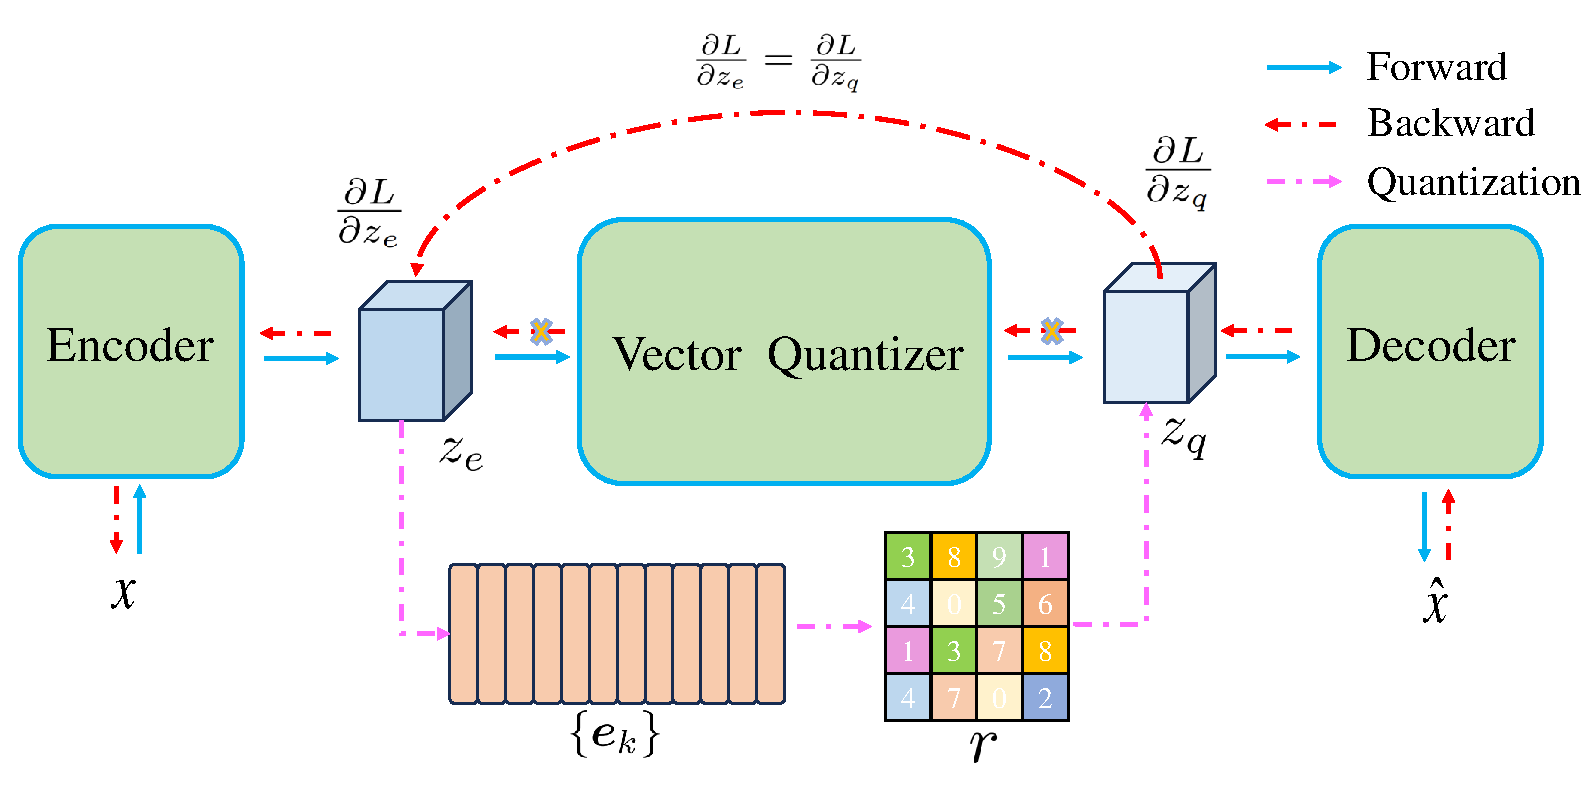
\includegraphics[width=1.0\textwidth]{figs/architecture/VQ.pdf}
\vspace{-4mm}
\caption{\small{The illustration of VQ.}}
\label{fig:vq model}
\end{center}
\end{wrapfigure} 
\fi

\begin{wrapfigure}[20]{r}{0.50\textwidth}
    \vspace{-6mm}
    \centering
    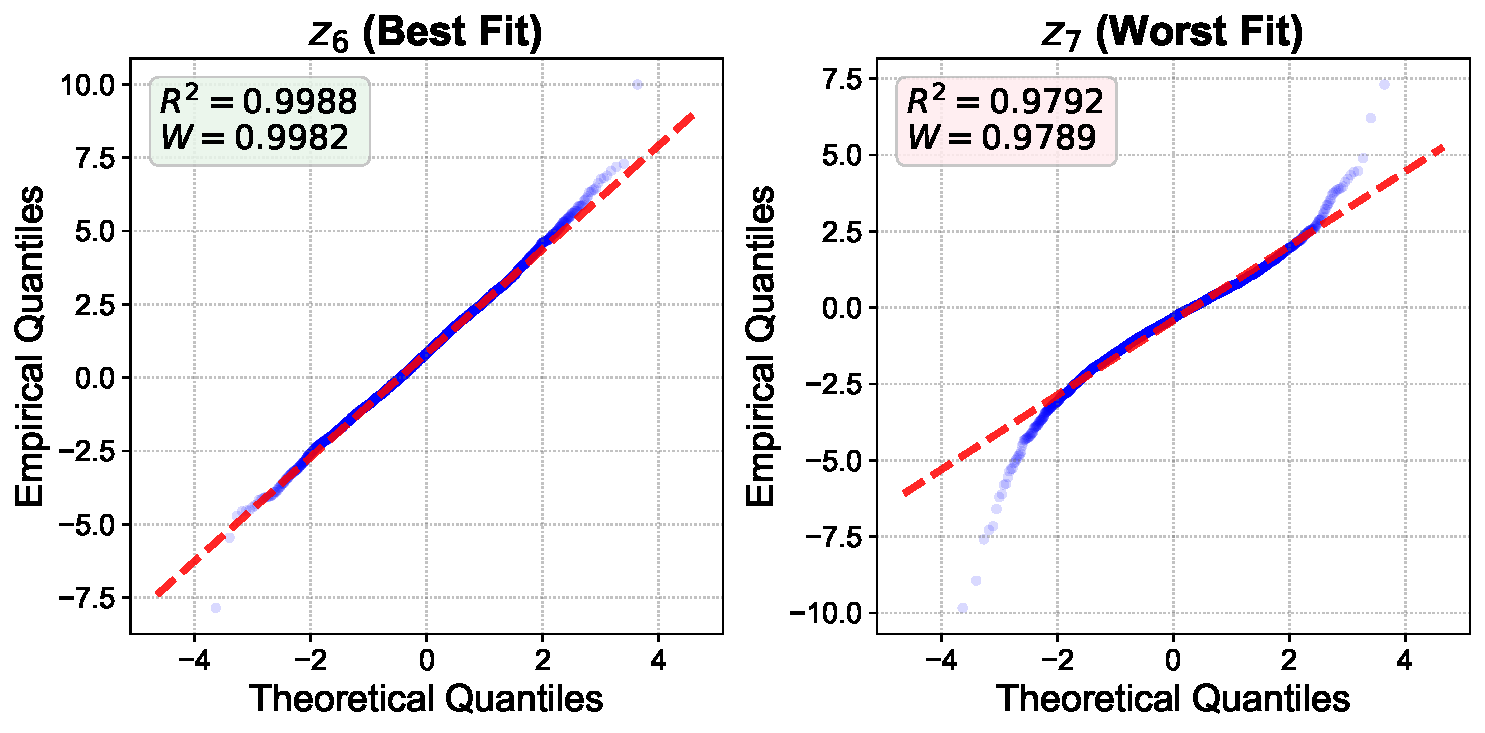
\includegraphics[width=0.98\linewidth]{figs/Gaussion/qq_plots_1d_main.pdf} 
    \vspace{-2mm}
    \caption{\textbf{Gaussianity Validation via Q-Q Plots.} We visualize the feature dimensions with the highest $z_6$ (Left) and lowest ($z_7$, Right) conformance to the Gaussian hypothesis. \textbf{Note:} For visual clarity, plots display a random subset of 5,000 points, while the reported statistics ($R^2, W$) are computed on the \textbf{full validation set ($N=409,600$)}. The strong alignment with the red identity line ($y=x$) confirms that the learned features are predominantly Gaussian, with deviations confined to sparse heavy tails.}
    \label{fig:qq_main}
    \vspace{-6mm}
\end{wrapfigure} 

\paragraph{Gaussian Approximation Validation}
To empirically assess the Gaussian approximation underlying our Wasserstein objective, we analyze the distributional properties of the learned latent features.
Using the FFHQ dataset, we extract latent vectors from a subset of 1,600 images ($d=8$), resulting in a total of $N=409{,}600$ samples.
Figure~\ref{fig:qq_main} presents Quantile--Quantile (Q--Q) plots for the feature dimensions exhibiting the highest ($z_6$) and lowest ($z_7$) agreement with a Gaussian reference.
Under an ideal Gaussian model, the samples (blue points) align with the theoretical reference line ($y=x$).
As shown, the best-fitting dimension ($z_6$) demonstrates near-perfect alignment, with a coefficient of determination of $R^2 = 0.9988$.
Importantly, even for the least-fitting dimension ($z_7$), the Q--Q plot evaluated over the distribution achieves a high goodness-of-fit score ($R^2 > 0.979$).
While mild deviations appear in the extreme tails, the central mass of the distribution, which dominates the probability mass and governs the Wasserstein objective, is well approximated by a Gaussian.
These results support the use of a Gaussian-based Wasserstein formulation as an effective approximation for distributional matching.
A more comprehensive univariate and multivariate analysis, including Mahalanobis distance based normality assessment across all dimensions, is provided in Appendix~\ref{sec:normality_tests}.



\begin{table*}[!t]
  \centering
  \caption{Analysis of generalization ability from ImageNet to FFHQ dataset.}
  \label{tab:generalization ability}
  \vspace{-1ex}
  \resizebox{\textwidth}{!}{%
  \begin{tabular}{@{}lccccccc@{}} \hline
    Approaches  & Tokens & Codebook Dim & $\mathcal{U}$ ({\color{green!60!black}\bfseries$\pmb{\uparrow}$}) & $\mathcal{C}$ ({\color{green!60!black}\bfseries$\pmb{\uparrow}$}) & PSNR({\color{green!60!black}\bfseries$\pmb{\uparrow}$}) & SSIM({\color{green!60!black}\bfseries$\pmb{\uparrow}$}) & Rec. Loss ({\color{green!60!black}\bfseries$\pmb{\downarrow}$})\\\hline
    Vanilla VQ & 256 & 16384 & 1.7\% & 332.9 & 27.18 & 71.6 & 0.0138\\ 							
    EMA VQ & 256 & 16384 & 12.5\% & 1292.1 & 27.69 & 72.3 & 0.0126 \\ 					
    Online VQ & 256 & 16384 & 33.2\% & 2794.9 & 27.91 & 72.7 & 0.0120 \\ 				
    \textbf{Wasserstein VQ} & 256 & 16384 & 99.2\% & 13975.4 & 28.62 & 75.0 &  0.0103 \\ 	
    \hline
    \vspace{-3ex}
  \end{tabular}
}
\end{table*}

\begin{table*}[!t]
  \centering
  \vspace{-1ex}
  \caption{The computational overhead of various VQ approaches.}
  \label{tab:computational overhead}
  \vspace{-1ex}
  \resizebox{\textwidth}{!}{%
  \begin{tabular}{@{}lcccccc@{}} \hline
    Approaches  & Codebook Size & Times (second)  & Codebook Size & Times (second)  & Codebook Size & Times (second) \\\hline
    Vanilla VQ & 16384 & \textbf{0.184} & 50000 & \textbf{0.408}  & 100000 & \textbf{0.655} \\ 
    EMA VQ & 16384 & 0.265 & 50000 & 0.807 & 100000 & 1.502\\  			
    Online VQ & 16384 & 1.810 & 50000 & 5.438 & 100000 & 10.64\\ 	
    \textbf{Wasserstein VQ} & 16384 & \underline{0.294}  & 50000 & \underline{0.525} & 100000& \underline{0.774} \\ 	
    \hline
    \vspace{-6ex}
  \end{tabular}
}
\end{table*}



\paragraph{Representation Visualization} 
To examine the learned distribution of feature and code vectors across different VQ methods trained on the FFHQ dataset (with a fixed codebook size of $K=8192$), we randomly sample 3,000 feature vectors and 1,000 code vectors and visualize them via scatter plots. As shown in Figures~\ref{fig:codebook_feature 1} and~\ref{fig:codebook_feature 2}, in both Vanilla VQ and EMA VQ, most code vectors are concentrated near the origin, rendering them largely inactive. While Online VQ mitigates this central clustering, its code vectors are pushed toward the extremes of the feature space, as illustrated in Figure~\ref{fig:codebook_feature 3}. This distributional mismatch leads to increased information loss and reduced codebook utilization. By contrast, \emph{Wasserstein VQ} achieves substantially better alignment between feature and code vector distributions, significantly reducing information loss and improving codebook utilization.

\begin{figure*}[!t]
    \vspace{-2mm}
	\centering
	\subfloat[Vanilla VQ]{ 
		\label{fig:codebook_feature 1}  
		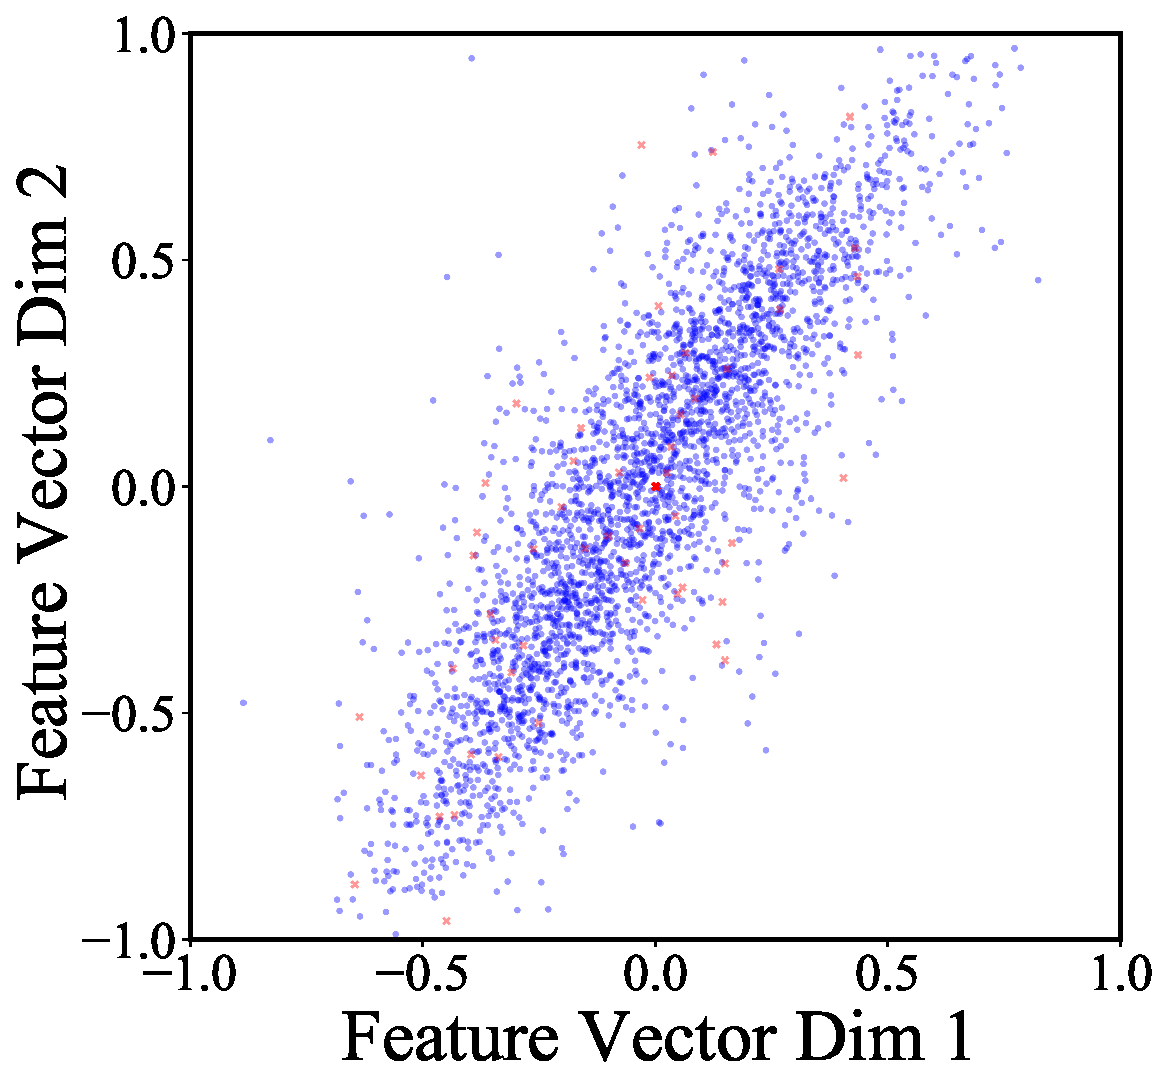
\includegraphics[width=0.225\textwidth]{figs/codebook_feature_visualization/vanilla_codebook_feature_visualization.pdf}
        }
	\hspace{0.03cm}
	\subfloat[EMA VQ]{
		\label{fig:codebook_feature 2}
		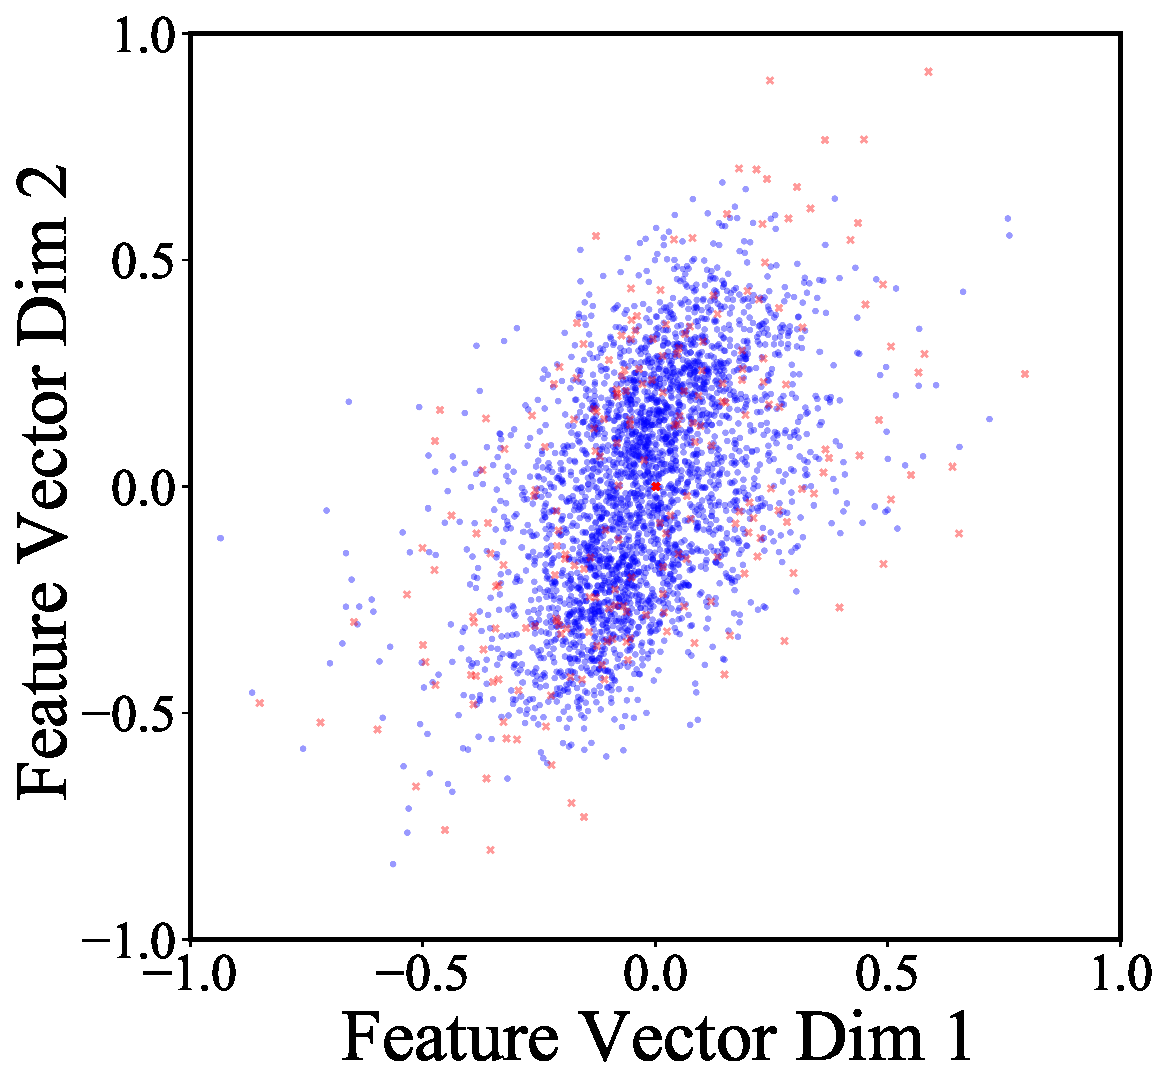
\includegraphics[width=0.225\textwidth]{figs/codebook_feature_visualization/ema_codebook_feature_visualization.pdf}
	}
        \hspace{0.03cm}
	\subfloat[Online VQ]{ 
		\label{fig:codebook_feature 3}  
		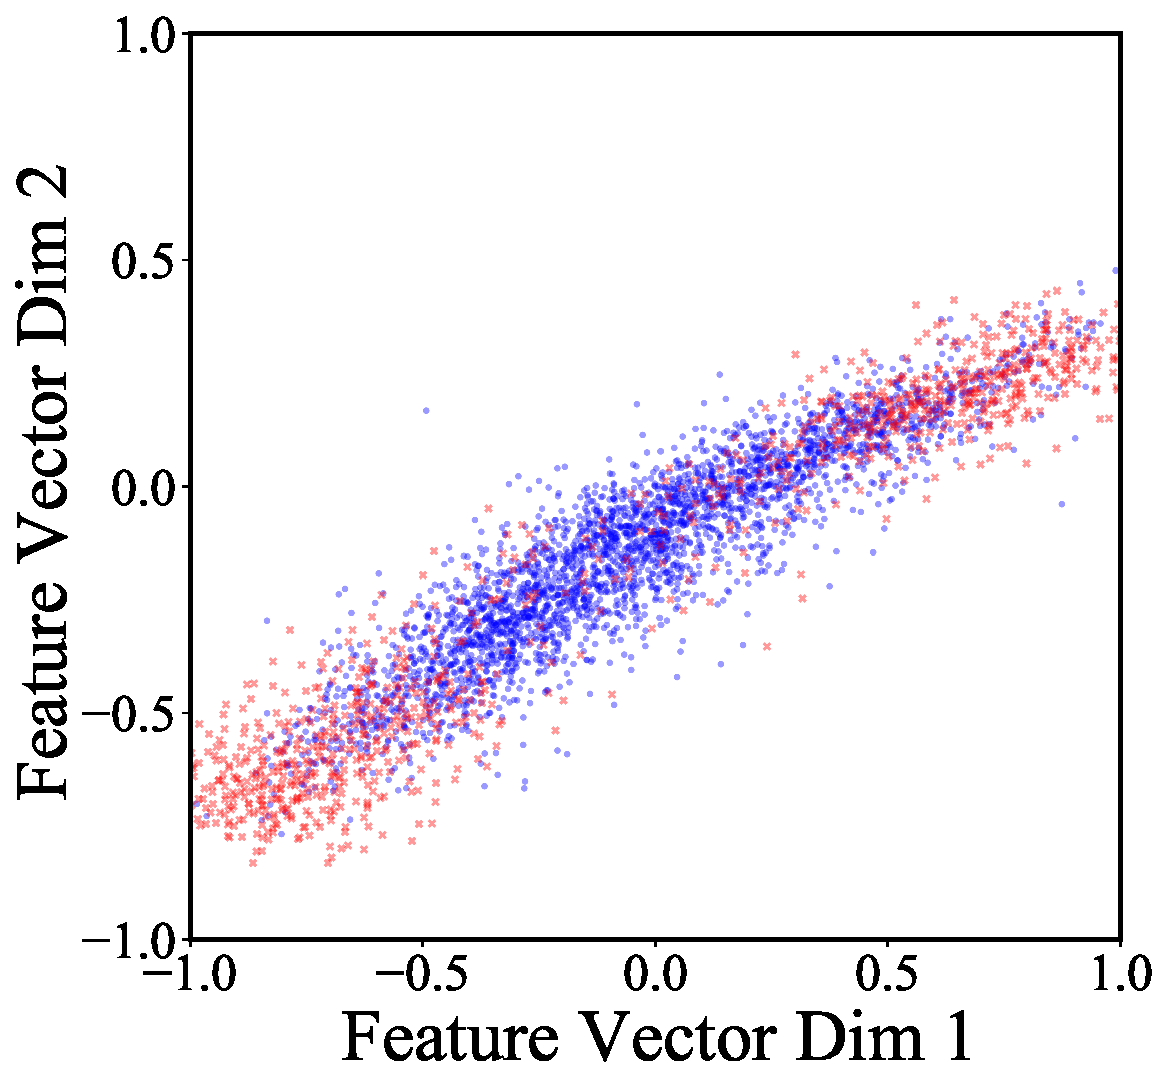
\includegraphics[width=0.225\textwidth]{figs/codebook_feature_visualization/online_codebook_feature_visualization.pdf}
	}
        \hspace{0.03cm}
	\subfloat[Wasserstein VQ]{
		\label{fig:codebook_feature 4}
		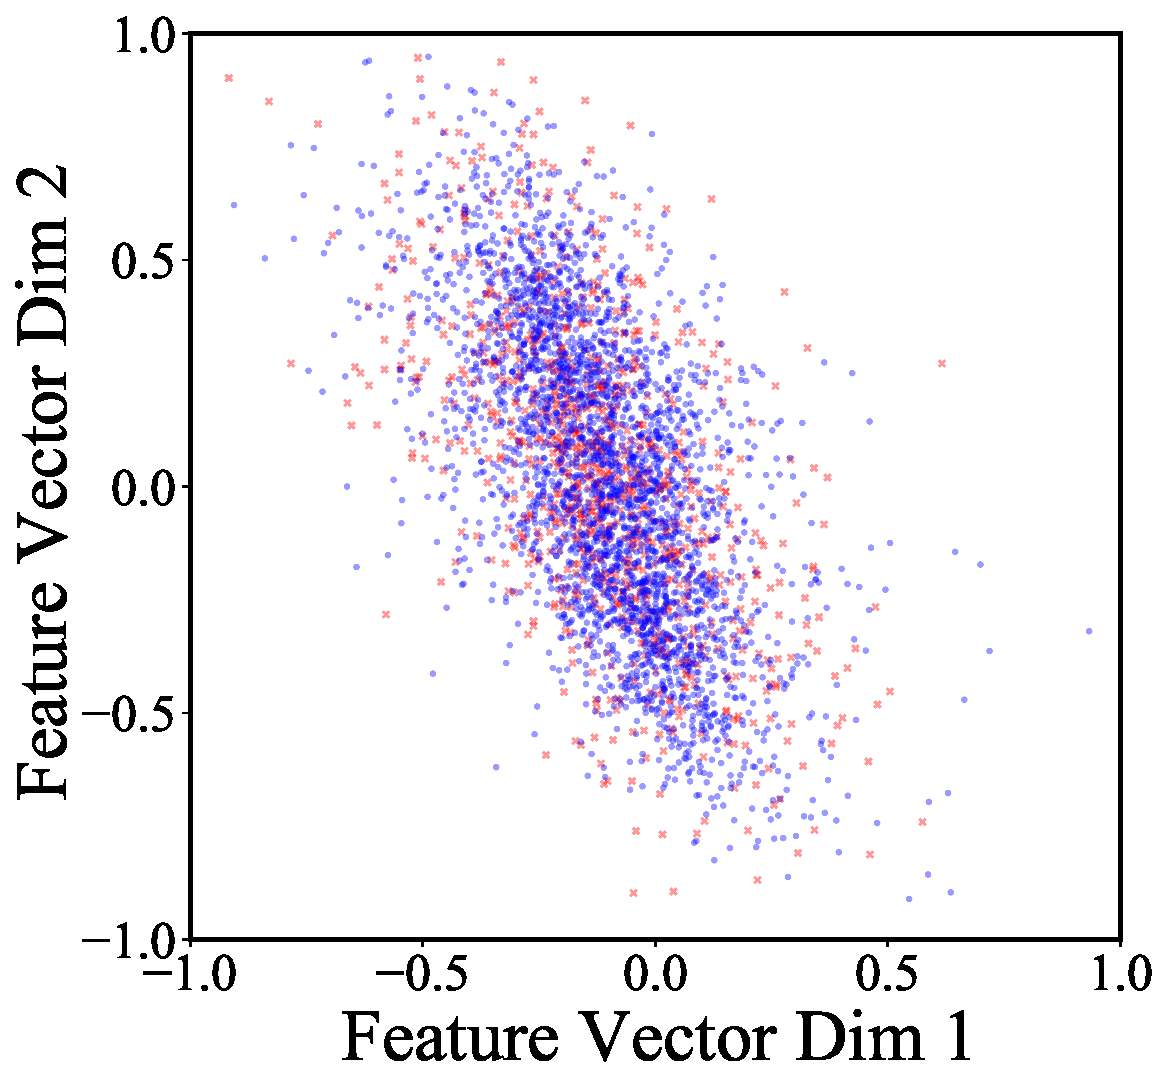
\includegraphics[width=0.225\textwidth]{figs/codebook_feature_visualization/wasserstein_codebook_feature_visualization.pdf}}
    \vspace{-2mm}
	\caption{Visualization of feature and codebook distributions. Blue $\cdot$ and red $\times$ represent the feature and code vectors, respectively.}
	\label{fig:feature codebook visualization}
    \vspace{-3mm}
\end{figure*}

\paragraph{Cross-Dataset Generalization}
To evaluate the model’s generalization capability, we conducted a cross-dataset transfer experiment. Specifically, we used the pre-trained checkpoint from Table~\ref{tab:vqvae imagenet} (trained on ImageNet) and evaluated its performance on the FFHQ dataset, which is out-of-distribution relative to ImageNet. The results are summarized in Table~\ref{tab:generalization ability}.

Among all methods, Wasserstein VQ achieves the highest performance in this transfer setting, indicating that the proposed distribution alignment objective does not impair generalization. Moreover, Wasserstein VQ’s strong performance on the out-of-distribution FFHQ dataset suggests that enforcing alignment may contribute to improved robustness under distribution shifts. Overall, these findings provide evidence that models trained with the proposed regularization generalize effectively to out-of-distribution data.


\paragraph{Computational Overhead Analyses} We evaluate the runtime efficiency by measuring the forward and backward pass times of the VQ module. As shown in Table~\ref{tab:computational overhead} in Appendix~\ref{appendix:computational overhead}, the runtime of Wasserstein VQ is comparable to Vanilla VQ, with only negligible overhead arising from the covariance computation.  This confirms that the closed-form Wasserstein objective offers a highly efficient pathway to optimal codebook utilization without incuring a significant time overhead. More implementation details see Appendix~\ref{appendix:computational overhead}.

\paragraph{Sensitivity Analysis on $\gamma$} 
We conduct a sensitivity analysis with respect to $\gamma$ on the FFHQ dataset by varying $\gamma \in \{0, 10^{-5}, 10^{-4}, 10^{-3}, 10^{-2}, 10^{-1}, 1\}$. As reported in Table~\ref{tab:sensitivity analysis} in Appendix~\ref{appendix:sensitivity analysis}, when $\gamma = 0$, Wasserstein VQ yields the worst performance, as it degenerates into the vanilla VQ formulation without distributional matching. As $\gamma$ increases from $10^{-5}$ to $10^{-3}$, the performance of Wasserstein VQ consistently improves. When $\gamma$ reaches $10^{-2}$, Wasserstein VQ achieves full ($100\%$) codebook utilization along with competitive quantitative results. Moreover, within the range $\gamma \in [10^{-2}, 1]$, the performance of Wasserstein VQ remains stable, indicating that the method is not sensitive to the precise choice of $\gamma$ once it exceeds a moderate threshold.



% \paragraph{Additional Analyses.} Due to space limitations, further analyses are deferred to the appendix. Specifically, Appendix~\ref{appendix:representation visualize} visualizes the feature and code distributions across different VQ methods. Appendix~\ref{appendix:sensitivity analysis} presents a sensitivity analysis w.r.t. $\gamma$. Appendix~\ref{appendix:generalization ability} demonstrates that Wasserstein VQ exhibits strong generalization from ImageNet to FFHQ in terms of reconstruction performance. Finally, Appendix~\ref{appendix:ablation study} shows that Wasserstein VQ scales more effectively to larger codebooks ($K=100{,}000$) and higher feature dimensions (e.g., $d=32$).

%\paragraph{Additional Analyses} Due to space limitations, additional analyses are provided in the appendix. Appendix~\ref{appendix:representation visualize} visualizes the feature and code distributions across different VQ methods, while Appendix~\ref{appendix:sensitivity analysis} presents a sensitivity analysis with respect to $\gamma$. Appendix~\ref{appendix:generalization ability} evaluates the generalization performance from ImageNet to FFHQ, and Appendix~\ref{appendix:ablation study} demonstrates that \emph{Wasserstein VQ} scales effectively to larger codebooks ($K=100{,}000$) and higher feature dimensions (e.g., $d=32$).

%\paragraph{Analyses of Codebook Size} We investigate the impact of the codebook size $K$  on the performance of VQ by varying across a wide range: $K \in [1024, 2048, 4096, 8192, 16384, 50000, 100000]$. As shown in Table~\ref{tab:vqvae ffhq},~\ref{tab:vqvae ffhq codebook size}, the vanilla VQ model suffers from severe codebook collapse even with a relatively small $K$, such as $K=1024$. In contrast, improved algorithms like EMA VQ and Online VQ can handle smaller codebook sizes effectively, but they still experience codebook collapse when $K$ is very large, e.g., $K\geq 50000$.
%Notably, the \emph{Wasserstein VQ} model consistently maintains 100\% codebook utilization, irrespective of the codebook size. This underscores the effectiveness of distributional matching via the quadratic Wasserstein distance in mitigating the issue of codebook collapse.

\paragraph{Effect of Codebook Size on FFHQ} To investigate the impact of codebook size on VQ performance, we vary the codebook size $K$  across a wide range: $K \in \{1024, 2048, 4096, 8192, 16384, 50000, 100000\}$. As shown in Table~\ref{tab:vqvae ffhq} in the main text and Table~\ref{tab:vqvae ffhq codebook size} in Appendix~\ref{appendix:ablation study}, the vanilla VQ model suffers from severe codebook collapse even at relatively small sizes, such as $K=1024$. In contrast, improved variants like EMA VQ and Online VQ handle smaller codebooks effectively, but still exhibit codebook collapse when $K$ becomes very large (e.g., $K \geq 50000$).  In contrast, \emph{Wasserstein VQ} consistently maintains 100\% codebook utilization across all codebook sizes, highlighting the effectiveness of enforcing distributional alignment via the quadratic Wasserstein distance in mitigating codebook collapse.

\paragraph{Effect of Codebook Dimensionality} 
We investigate the impact of codebook dimensionality on VQ performance by conducting experiments on CIFAR-10 with $d$ ranging from 2 to 32. As reported in Table~\ref{tab:vqvae cifar-10 codebook dimension} (Appendix~\ref{appendix:ablation study}), our proposed Wasserstein VQ consistently outperforms all baselines across all dimensionalities. We also observe a manifestation of the curse of dimensionality: performance generally degrades as $d$ increases. Vanilla VQ experiences the most severe decline, followed by EMA VQ and Online VQ, whereas Wasserstein VQ exhibits only minimal reduction in codebook utilization.

%\paragraph{Effect of Codebook Dimensionality} We finally investigate the impact of codebook dimensionality on VQ performance. Conducting experiments on CIFAR-10 with dimensionality $d$ ranging from 2 to 32, our proposed Wasserstein VQ consistently outperforms all baselines regardless of dimensionality, as shown in Table~\ref{tab:vqvae cifar-10 codebook dimension} in Appendix~\ref{appendix:ablation study}. Notably, we observe the curse of dimensionality phenomenon—performance degrades as dimensionality increases. Vanilla VQ exhibits the most severe degradation, followed by EMA VQ and Online VQ, while our Wasserstein VQ shows only minimal codebook utilization reduction.

\begin{table*}[!t]
\centering
\vspace{-1ex}
\caption{
    {Reconstruction performance on the ImageNet-1K dataset. The suffixes "–a," "–b," and "–c" correspond to decoder adaptation for 5, 10, and 15 epochs, respectively. The best-performing result is highlighted in bold. Results marked with $^{\dagger}$ are cited from VQGAN-LC \cite{Zhu2024ScalingTC}, those with $^{\star}$ from Llama GEN \cite{Sun2024AutoregressiveMB}, and those with $^{\ddagger}$ from VQ-Transplant \cite{Fang2025VQTransplant}. }
    }
\vspace{-1ex}
\small
\resizebox{0.97\textwidth}{!}{
\begin{tabular}{@{}lcccccccc@{}}
\toprule
\textbf{Methods} & \textbf{Tokens} & \textbf{Codebook Size} & $\mathcal{U}$ ({\color{green!60!black}\bfseries$\pmb{\uparrow}$}) & \textbf{r-FID} ({\color{green!60!black}\bfseries$\pmb{\downarrow}$}) & \textbf{r-IS} ({\color{green!60!black}\bfseries$\pmb{\uparrow}$}) & \textbf{LPIPS} ({\color{green!60!black}\bfseries$\pmb{\downarrow}$}) & \textbf{PSNR} ({\color{green!60!black}\bfseries$\pmb{\uparrow}$}) & \textbf{SSIM} ({\color{green!60!black}\bfseries$\pmb{\uparrow}$})\\
\midrule
DQVAE$^{\dagger}$ & 256  & $1{,}024$& - & 4.08  & - & - & - & - \\
DiVAE$^{\dagger}$ & 256 & $16{,}384$ & - & 4.07 & - & - & - & - \\
RQVAE$^{\dagger}$ & 256 & $16{,}384$ & - &  3.20 & - & - & - & -\\
RQVAE$^{\dagger}$ & 512 & $16{,}384$ & - & 2.69 & - & - & - & -\\
RQVAE$^{\dagger}$ & $1{,}024$& $16{,}384$ & - & 1.83 & - & - & -  & -\\
DF-VQGAN$^{\dagger}$ & 256 & $12{,}288$ & - & 5.16 & - & - & - & - \\
DF-VQGAN$^{\dagger}$ & $1{,}024$& $8{,}192$& - & 1.38 & - & - & - & - \\
Llama GEN$^{\star}$ & 256 & $16{,}384$ & 97.0\% & 2.19 & -  & - &  20.79 & 67.5 \\
\midrule
\multirow{3}{*}{VQGAN$^{\dagger}$}  & 256 & $16{,}384$ & 3.4\% & 5.96 & - & 0.17 & 23.3& 52.4 \\
& 256 &  $50{,}000$ & 1.1\% & 5.44 & - & 0.17 & 22.5 & 52.5 \\
& 256 &  $100{,}000$ & 0.5\% &  5.44 & - & 0.17 & 22.3 & 52.5 \\
\midrule
\multirow{3}{*}{VQGAN-FC$^{\dagger}$} & 256 & $16{,}384$ & 11.2\%  & 4.29 & - & 0.17 & 22.8 & 54.5 \\ 
& 256 & $50{,}000$ & 3.6\%  & 4.96 & - & 0.15 & 23.1 & 54.7 \\
& 256 & $100{,}000$ & 1.9\%  & 4.65 & - & 0.15 & 22.9 & 55.1 \\
\midrule
\multirow{3}{*}{VQGAN-EMA$^{\dagger}$} & 256 & $16{,}384$ & 83.2\% & 3.41 & -  & 0.14 & 23.5 & 56.6 \\
& 256 & $50{,}000$ &  40.2\% & 3.88 & -  & 0.14 & 23.2 & 55.9 \\
& 256 & $100{,}000$ & 24.2\% & 3.46 & -  &  0.13 & 23.4 & 56.2 \\
\midrule
\multirow{4}{*}{VQGAN-LC$^{\dagger}$} & 256 & $16{,}384$ & \textbf{99.9\%}  & 3.01 & - & 0.13 & 23.2 & 56.4 \\
 & 256 & $50{,}000$ & \textbf{99.9\%}  & 2.75 & - & 0.13 &  23.8 &  58.4 \\
 & 256 & $100{,}000$ & \textbf{99.9\%}  & 2.62 & - &  0.12 &  23.8 & 58.9 \\
 & $1{,}024$& $100{,}000$ & 99.5\%  & 1.29 & - &  \textbf{0.07} &  \textbf{27.0} &  \textbf{71.6} \\\midrule
\midrule
\multirow{3}{*}{\textbf{Wasserstein VQ-a}$^{\ddagger}$} & 512 & $16{,}384$ & 99.8\% & 1.04 & 191.3 & 0.114 & 24.36 & 64.0 \\
& 512 & $32{,}768$&  99.7\% & 0.98 &  193.9 & 0.111 & 24.37 & 64.3 \\
& 512 & $65{,}536$& 99.6\% & 0.92 & 195.5 & 0.106 & 24.68 & 65.4 \\\midrule
\multirow{3}{*}{\textbf{Wasserstein VQ-b}} & 512 & $16{,}384$ & 99.8\% & 0.98 & 192.9 & 0.114 & 24.34 & 63.7\\
& 512 & $32{,}768$& 99.8\% & 0.88 & 196.2 & 0.109 & 24.60 & 64.7 \\
& 512 & $65{,}536$& 99.6\% & 0.81 & \textbf{198.7} & 0.105 & \textbf{24.77} & \textbf{65.5}\\\midrule
\multirow{3}{*}{\textbf{Wasserstein VQ-c}} & 512 & $16{,}384$ & 99.8\% & 0.90 & 194.1 & 0.114 & 24.27 & 63.4\\
& 512 & $32{,}768$& 99.8\% & 0.85 & 196.4 & 0.109 & 24.43 & 64.1 \\
& 512 & $65{,}536$& 99.6\% & \textbf{0.79} & 198.5 & \textbf{0.104} & 24.73 & 65.2 \\
\bottomrule
\end{tabular}}
\vspace{-3ex}
\label{tab:reconstruction_IN-main table}
\end{table*}

\begin{table}[!t]
\centering
\caption{
    {Reconstruction performance on the ImageNet-1K dataset for multi-scale quantization algorithms. The suffixes "–a," "–b," and "–c" correspond to decoder adaptation for 5, 10, and 15 epochs, respectively. For each codebook size, the best-performing result is highlighted in bold. $^{\ddagger}$: results are cited from VQ-Transplant \cite{Fang2025VQTransplant}. }
    }
\small
\resizebox{0.97\textwidth}{!}{
\begin{tabular}{@{}lcccccc@{}}
\toprule
\textbf{Methods} & \textbf{Tokens} & \textbf{Codebook Size} & $\mathcal{E}$ ({\color{green!60!black}\bfseries$\pmb{\downarrow}$}) & $\mathcal{U}$ ({\color{green!60!black}\bfseries$\pmb{\uparrow}$}) & $\mathcal{C}$ ({\color{green!60!black}\bfseries$\pmb{\uparrow}$}) & \textbf{r-FID} ({\color{green!60!black}\bfseries$\pmb{\downarrow}$}) \\\midrule
VAR$^{\ddagger}$ & 680 & $4{,}096$& 0.283 & \textbf{100\%} & $2{,}981.4$ & 0.92\\\midrule
\multirow{2}{*}{Vanilla VAR-a$^{\ddagger}$} & 680 & $4{,}096$& 0.305 & 38.2\% & $1{,}300$.4 & 1.25 \\
& 680 & $8{,}192$& 0.309 & 22.9\% & $1{,}422$.6 & 1.30\\\midrule
\multirow{2}{*}{EMA VAR-a$^{\ddagger}$} & 680 & $4{,}096$& 0.321 & 99.9\% & $1{,}806$.6 &  1.69 \\
& 680 & $8{,}192$&  0.312 & 99.8\% & $2{,}498$.8 &  1.15\\\midrule
\multirow{2}{*}{Online VAR-a$^{\ddagger}$} & 680 & $4{,}096$&  0.276 &  99.0\% & $1{,}950$.9 & 1.05\\
& 680 & $8{,}192$& 0.269 & 73.9\% & $3{,}588$.6 & 1.00\\\midrule
\multirow{2}{*}{\textbf{Wasserstein VAR-a}$^{\ddagger}$} & 680 & $4{,}096$& \textbf{0.255} & \textbf{100\%} &  \textbf{$3{,}286.2$} & 0.93 \\
& 680 & $8{,}192$&  \textbf{0.240}  & \textbf{100\%} & \textbf{$6{,}518.2$}
 & 0.83\\\midrule
\multirow{2}{*}{\textbf{Wasserstein VAR-b}} & 680 & $4{,}096$& \textbf{0.255} & \textbf{100\%} & \textbf{$3{,}286.2$} & 0.88 \\
& 680 & $8{,}192$&  \textbf{0.240}  & \textbf{100\%} & \textbf{$6{,}518.2$}
 & 0.79 \\\midrule
\multirow{2}{*}{\textbf{Wasserstein VAR-c}} & 680 & $4{,}096$& \textbf{0.255} & \textbf{100\%} & \textbf{$3{,}286.2$} & \textbf{0.81} \\
& 680 & $8{,}192$&  \textbf{0.240}  & \textbf{100\%} & \textbf{$6{,}518.2$}
 & \textbf{0.73}\\
\bottomrule
\end{tabular}}
\vspace{-4ex}
\label{tab:reconstruction_IN-multi-scale}
\end{table}


\subsection{Evaluation on the VQGAN Framework}
%We evaluate the proposed method on the ImageNet and FFHQ datasets under the VQGAN framework.
%On ImageNet, we compare against a broad range of representative vector quantization approaches,
%including classical VQ-based models (VQGAN~\cite{Esser2020TamingTF}, VQGAN-FC~\cite{Yu2021VectorquantizedIM}, VQGAN-EMA~\cite{Razavi2019GeneratingDH}),
%hierarchical and residual variants (RQVAE~\cite{Lee2022AutoregressiveIG}, DiVAE~\cite{Shi2022DiVAEPI}),
%recent large-codebook and scaling-oriented methods (VQGAN-LC~\cite{Zhu2024ScalingTC}, VAR~\cite{Tian2024VisualAM}),
%as well as strong autoregressive tokenizers (Llama GEN~\cite{Sun2024AutoregressiveMB}, DQVAE~\cite{Huang2023TowardsAI}, DF-VQGAN~\cite{Ni2022NWALIPLI}). 
%For FFHQ, we evaluate against RQVAE~\cite{Lee2022AutoregressiveIG}, VQGAN~\cite{Esser2020TamingTF}, VQGAN-FC~\cite{Yu2021VectorquantizedIM}, VQGAN-EMA~\cite{Razavi2019GeneratingDH}, VQ-WAE~\cite{Vuong2023VectorQW}, MQVAE~\cite{Huang2023NotAI}, and VQGAN-LC~\cite{Zhu2024ScalingTC}.

\paragraph{Datasets and Baselines} We evaluate our proposed method against a comprehensive set of baselines on the ImageNet and FFHQ datasets. For ImageNet, the compared methods include DQVAE~\cite{Huang2023TowardsAI}, DF-VQGAN~\cite{Ni2022NWALIPLI}, DiVAE~\cite{Shi2022DiVAEPI}, RQVAE~\cite{Lee2022AutoregressiveIG}, VQGAN~\cite{Esser2020TamingTF}, VQGAN-FC~\cite{Yu2021VectorquantizedIM}, VQGAN-EMA~\cite{Razavi2019GeneratingDH}, VQGAN-LC~\cite{Zhu2024ScalingTC}, Llama GEN~\cite{Sun2024AutoregressiveMB}, and VAR~\cite{Tian2024VisualAM}.
For FFHQ, we compare against RQVAE~\cite{Lee2022AutoregressiveIG}, VQGAN~\cite{Esser2020TamingTF}, VQGAN-FC~\cite{Yu2021VectorquantizedIM}, VQGAN-EMA~\cite{Razavi2019GeneratingDH}, VQ-WAE~\cite{Vuong2023VectorQW}, MQVAE~\cite{Huang2023NotAI}, and VQGAN-LC~\cite{Zhu2024ScalingTC}. Implementation details see Appendix~\ref{appendix:experimental details}.

\paragraph{Metrics} We report standard reconstruction and perceptual quality metrics, including Fréchet Inception Distance (r-FID)~\cite{Heusel2017GANsTB},
Reconstruction Inception Score (r-IS)~\cite{Salimans2016ImprovedTF},
Learned Perceptual Image Patch Similarity (LPIPS)~\cite{Zhang2018TheUE},
Peak Signal-to-Noise Ratio (PSNR), and Structural Similarity Index Measure (SSIM).



% \paragraph{Main Results.} As shown in Table~\ref{tab:reconstruction_IN-main table} and Table~\ref{tab:vqgan tranplant ffhq} in Appendix~\ref{appendix:supplement results on ffhq}, our proposed \emph{Wasserstein VQ} achieves the lowest r-FID within the VQGAN framework, demonstrating that VQ algorithms based on distribution matching can achieve superior reconstruction fidelity and perceptual quality. We further evaluate multi-scale quantization algorithms in Table~\ref{tab:reconstruction_IN-multi-scale}. Notably, all experiments in this table are fully controlled: the encoder–decoder architecture is identical to VAR~\cite{Tian2024VisualAM}, and, crucially, the latent features are kept fixed across all methods, ensuring that measurements of the criterion triple are unaffected by latent feature variance, as discussed in Appendix~\ref{appendix:Impact of Distribution Variance}. Under these controlled conditions, our \emph{Wasserstein VAR} achieves the best performance across the entire criterion triple, particularly yielding the lowest quantization error. Reconstruction performance further improves as we increase the number of decoder adaptation epochs, corresponding to stronger adversarial refinement; for example, for $K=8192$, the r-FID decreases steadily from \textbf{0.83} for Wasserstein VAR-a to \textbf{0.73} for Wasserstein VAR-c. Visualizations in Figures~\ref{fig:visual reconstruction ffhq} and~\ref{fig:visual reconstruction imagenet} (Appendix~\ref{appendix:reconstruction visualization}) show that the reconstructions produced by our approach remain nearly indistinguishable from the original inputs, confirming its strong visual tokenization capability.
% \vspace{-1ex}

\begin{table*}[!t]
\centering
\caption{{Reconstruction performance on the FFHQ dataset. Results marked with $^{\dagger}$ are cited from VQGAN-LC \cite{Zhu2024ScalingTC}, and those with $^{\ddagger}$ from VQ-Transplant~\cite{Fang2025VQTransplant}.}}
\vspace{-1ex}
\label{tab:vqgan tranplant ffhq}
\resizebox{0.96\textwidth}{!}{%
\begin{tabular}{@{}lcccccccc@{}}
\toprule
VQs & Tokens & Codebook Size $K$ & $\mathcal{E}$({\color{green!60!black}\bfseries$\pmb{\downarrow}$}) & $\mathcal{U}$ ({\color{green!60!black}\bfseries$\pmb{\uparrow}$}) & PSNR({\color{green!60!black}\bfseries$\pmb{\uparrow}$}) & SSIM({\color{green!60!black}\bfseries$\pmb{\uparrow}$}) & LPIPS ({\color{green!60!black}\bfseries$\pmb{\downarrow}$}) & r-FID({\color{green!60!black}\bfseries$\pmb{\downarrow}$}) \\
\midrule
RQVAE$^{\dagger}$ & 256 & 2048 & - & - & 22.9 & 67.0 & 0.13 & 7.04  \\
VQ-WAE$^{\dagger}$ & 256 & 1024 & - & -  & 22.5 & 66.5 & 0.12 & 4.20 \\
MQVAE$^{\dagger}$ & 256 & 1024 & - & 78.2\% & - & - & -  & 4.55 \\
VQGAN$^{\dagger}$ & 256 & 16384 & - & 2.3\% & 24.4 & 63.3 & 0.12 & 5.25  \\
VQGAN-FC$^{\dagger}$ & 256 & 16384  & - & 10.9\% & 24.8 & 64.6 & 0.11 & 4.86  \\
VQGAN-EMA$^{\dagger}$  & 256 & 16384  & - & 68.2\% & 25.4 & 66.1 & 0.10 & 4.79   \\
VQGAN-LC$^{\dagger}$ & 256 & 100000  & - & 99.5\% & 26.1 & 69.4 & 0.08 & 3.81   \\\midrule
\textbf{Wasserstein VQ$^{\ddagger}$} & 512 & 16384 & \textbf{0.153} & \textbf{99.7\%}   &  \textbf{27.25} & \textbf{75.4} & \textbf{0.075} & \textbf{1.81} \\
\textbf{Wasserstein VQ$^{\ddagger}$} & 512 & 32768  & \textbf{0.142} & \textbf{99.7\%}  & \textbf{27.33} & \textbf{75.7} & \textbf{0.072} & \textbf{1.21} \\
\bottomrule
\vspace{-4ex}
\end{tabular}
}
\end{table*}

\begin{figure*}[!t]
    \centering
    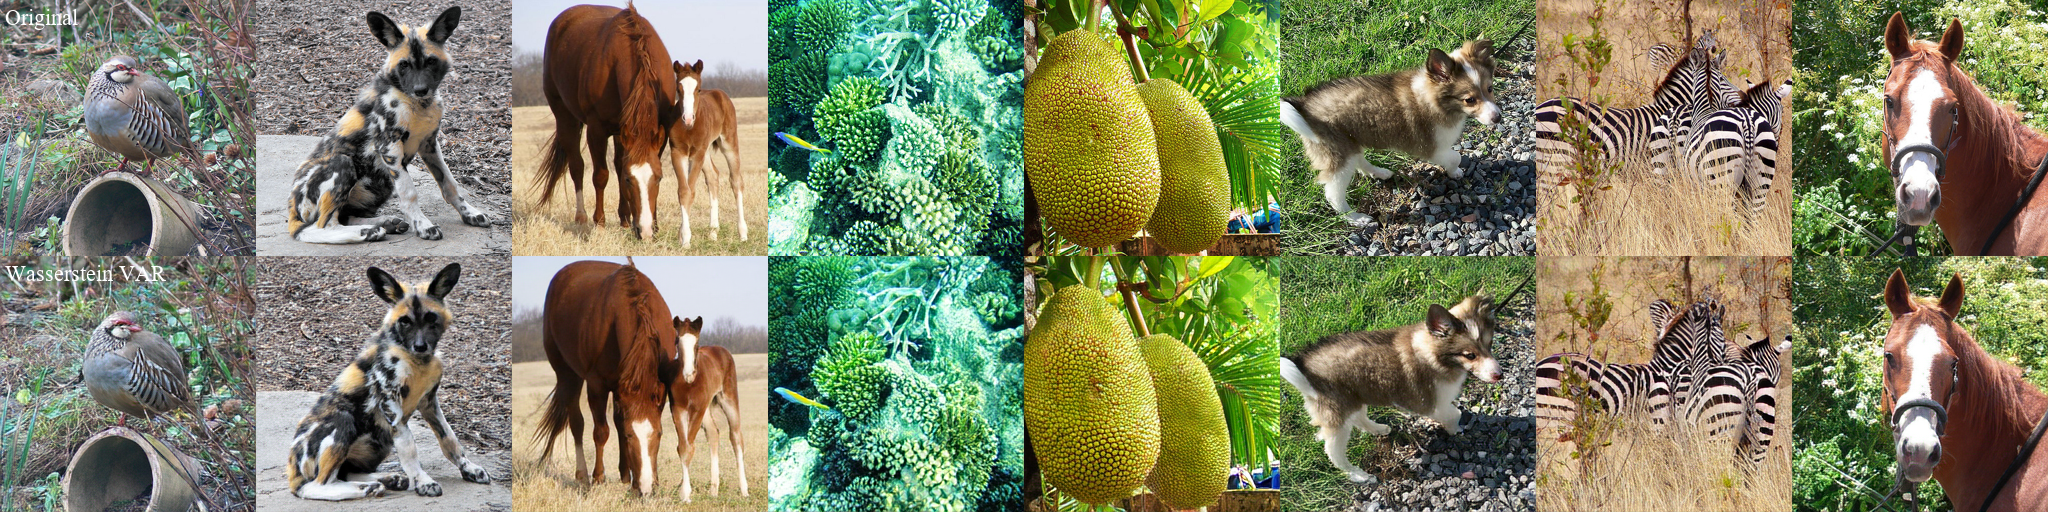
\includegraphics[width=0.96\linewidth]{figs/reconstruction/VAR_Visualization_On_ImageNet.png}
    \vspace{-1ex}
    \caption{Visualization of reconstructed ImageNet Images. The top row displays the original input images with a resolution of $256 \times 256$ pixels, while the bottom row shows the reconstructed images from the \emph{Wasserstein VAR}.}
    \label{fig:visual reconstruction imagenet}
    \vspace{-2ex}
\end{figure*}

\begin{figure*}[!t]
    \centering    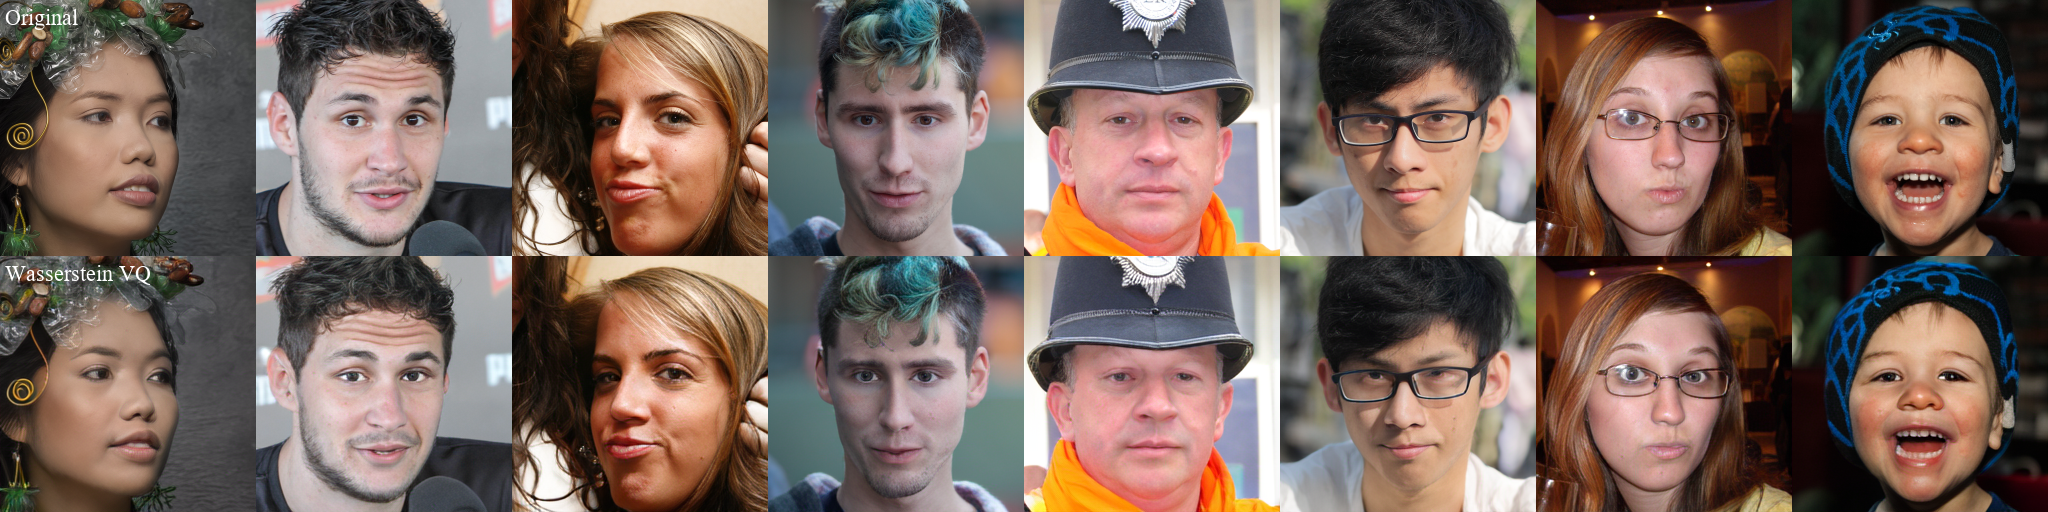
\includegraphics[width=0.96\linewidth]{figs/reconstruction/VQ_Visualization_On_FFHQ.png}
    \vspace{-1ex}
    \caption{Visualization of reconstructed FFHQ Images. The top row displays the original input images with a resolution of $256 \times 256$ pixels, while the bottom row shows the reconstructed images from the \emph{Wasserstein VQ}.}
    \label{fig:visual reconstruction ffhq}
    \vspace{-3ex}
\end{figure*}

\paragraph{Main Results} As shown in Tables~\ref{tab:reconstruction_IN-main table} and~\ref{tab:vqgan tranplant ffhq}, our proposed \emph{Wasserstein VQ} achieves the lowest r-FID within the VQGAN framework. %This indicates that explicitly aligning distributions not only reduces distortion but also provides a more faithful representational foundation for generative modeling. 
We further evaluate multi-scale quantization algorithms in Table~\ref{tab:reconstruction_IN-multi-scale}. All experiments in this table are conducted under fully controlled conditions: the encoder–decoder architecture is fixed to VAR~\cite{Tian2024VisualAM}, and, importantly, the latent features are kept identical across all methods. This ensures that measurements of codebook utilization, perplexity, and quantization error are not influenced by variations in the latent features, as discussed in Section~\ref{sec:distributional formulation}.

Under these controlled conditions, \emph{Wasserstein VAR} consistently demonstrates the strongest overall performance, with particularly notable improvements in quantization error. Reconstruction quality further improves as the number of decoder adaptation epochs increases, reflecting stronger adversarial refinement. For instance, when $K=8192$, the r-FID decreases from \textbf{0.83} (Wasserstein VAR-a) to \textbf{0.73} (Wasserstein VAR-c).

%\paragraph{Main Results} As shown in Tables~\ref{tab:reconstruction_IN-main table}, and~\ref{tab:vqgan tranplant ffhq},
%our proposed \emph{Wasserstein VQ} achieves the lowest r-FID within the VQGAN framework.
%This demonstrates that explicitly aligning distributions not only reduces distortion,
%but also provides a higher-fidelity representational foundation for generative modeling. We further evaluate multi-scale quantization algorithms in Table~\ref{tab:reconstruction_IN-multi-scale}.
%All experiments in this table are conducted under fully controlled conditions:
%the encoder--decoder architecture is fixed to VAR~\cite{Tian2024VisualAM},
%and, crucially, the latent features are kept fixed across all methods.
%This ensures that measurements of codebook utilization, perplexity, and quantization error
%are not confounded by latent feature variance,
%as analyzed in Appendix~\ref{appendix:Impact of Distribution Variance}.

%Under these controlled conditions, \emph{Wasserstein VAR} consistently achieves the strongest overall performance, with particularly notable improvements in quantization error.
%Reconstruction quality further improves as the number of decoder adaptation epochs increases,
%corresponding to stronger adversarial refinement; for example, for $K=8192$, the r-FID decreases from \textbf{0.83} for Wasserstein VAR-a to \textbf{0.73} for Wasserstein VAR-c.


\paragraph{Reconstruction Visualization}
To further demonstrate the reconstruction performance, we visualize the reconstructed FFHQ and ImageNet images in Figure~\ref{fig:visual reconstruction ffhq} and~\ref{fig:visual reconstruction imagenet}. As shown, the images reconstructed by our method are nearly identical to the original inputs. In particular, on the FFHQ dataset, only very minor differences can be observed in fine details. 
\vspace{-1ex}

\begin{table}[!t]
\centering
\caption{
    {Reconstruction performance on the ImageNet-1K dataset for multi-scale quantization algorithms. The suffixes “–a,” “–b,” and “–c” correspond to decoder adaptation for 5, 10, and 15 epochs, respectively. For each codebook size, the best-performing result is highlighted in bold. }
    }
%\vspace*{-5pt}
\resizebox{0.95\textwidth}{!}{
\begin{tabular}{@{}lcccccccc@{}}
\toprule
Methods & Tokens  & Codebook Size $K$ & $\mathcal{E}$ ({\color{green!60!black}\bfseries$\pmb{\downarrow}$}) & $\mathcal{U}$ ({\color{green!60!black}\bfseries$\pmb{\uparrow}$}) & $\mathcal{C}$ ({\color{green!60!black}\bfseries$\pmb{\uparrow}$}) & r-FID ({\color{green!60!black}\bfseries$\pmb{\downarrow}$}) \\\midrule
\multirow{2}{*}{MMD VAR-a} & 680 & 4096 & \textbf{0.255} & \textbf{100\%} & \textbf{3757.3}  &   \textbf{0.91}\\
& 680 & 8192 &  \textbf{0.234}  & \textbf{100\%} & \textbf{7539.4} &  \textbf{0.81}\\
\multirow{2}{*}{\textbf{Wasserstein VAR-a}} & 680 & 4096 & \textbf{0.255} & \textbf{100\%} &  3286.2 & 0.93 \\
& 680 & 8192 &  0.240  & \textbf{100\%} & 6518.2
 & 0.83\\\midrule
\multirow{2}{*}{MMD VAR-b} & 680 & 4096 & \textbf{0.255} & \textbf{100\%} & \textbf{3757.3}  &  \textbf{0.87}\\
& 680 & 8192 &   \textbf{0.234} & \textbf{100\%} & \textbf{7539.4} 
 & \textbf{0.78}\\
\multirow{2}{*}{\textbf{Wasserstein VAR-b}} & 680 & 4096 & \textbf{0.255} & \textbf{100\%} & 3286.2 & 0.88 \\
& 680 & 8192 &  0.240 & \textbf{100\%} & 6518.2
 & 0.79 \\\midrule
\multirow{2}{*}{MMD VAR-c} & 680 & 4096 & \textbf{0.255} & \textbf{100\%} & \textbf{3757.3}  &   0.82\\
& 680 & 8192 &  \textbf{0.234}  & \textbf{100\%} & 
 \textbf{7539.4} & 0.75\\
\multirow{2}{*}{\textbf{Wasserstein VAR-c}} & 680 & 4096 & \textbf{0.255} & \textbf{100\%} & 3286.2 & \textbf{0.81} \\
& 680 & 8192 &  0.240  & \textbf{100\%} & 6518.2
 & \textbf{0.73}\\
\bottomrule
\end{tabular}}
\vspace{-1.5ex}
\label{tab:mmd vs wasserstein}
\end{table}


\section{Discussion on Two Distributional Matching Approaches: Wasserstein VQ vs. MMD VQ}
\label{sec:mmd-vs-wasserstein}

We compare Wasserstein VQ and MMD VQ from three perspectives: visual tokenization performance, computational efficiency, and robustness to non-Gaussian distributions. First, we assess visual tokenization performance under the VQGAN framework. As shown in Table~\ref{tab:mmd vs wasserstein}, we evaluate performance with decoder adaptation conducted for 5, 10, and 15 epochs. Overall, the two methods achieve very similar performance, with Wasserstein VQ slightly outperforming MMD VQ when the decoder adaptation is extended to 15 epochs.

Second, we analyze the computational cost of the two approaches. Following the setup in Appendix~\ref{appendix:computational overhead}, we measure runtime efficiency by recording forward and backward pass times over 100 iterations. We consider two scenarios: (i) fixing the number of data samples at $N = 8192$ while varying the codebook size $K$ from 128 to 32,768, and (ii) fixing the codebook size at $K = 8192$ while varying the number of data samples $N$ from 128 to 32,768, providing complementary comparisons. As illustrated in Figures~\ref{fig:computational-codebook} and~\ref{fig:computational-data}, MMD VQ exhibits a rapidly increasing computational cost, reflecting its inefficiency. This difference arises because Wasserstein VQ performs distribution matching by aligning first- and second-order statistics, whereas MMD VQ relies on pairwise distances between all elements. Consequently, the computational complexity of MMD VQ grows substantially, especially when both the number of data samples and the codebook size are large.

\begin{figure}[!t]
	\centering
    %\vspace{-2mm}
	\subfloat[Codebook Size]{ 
		\label{fig:computational-codebook}  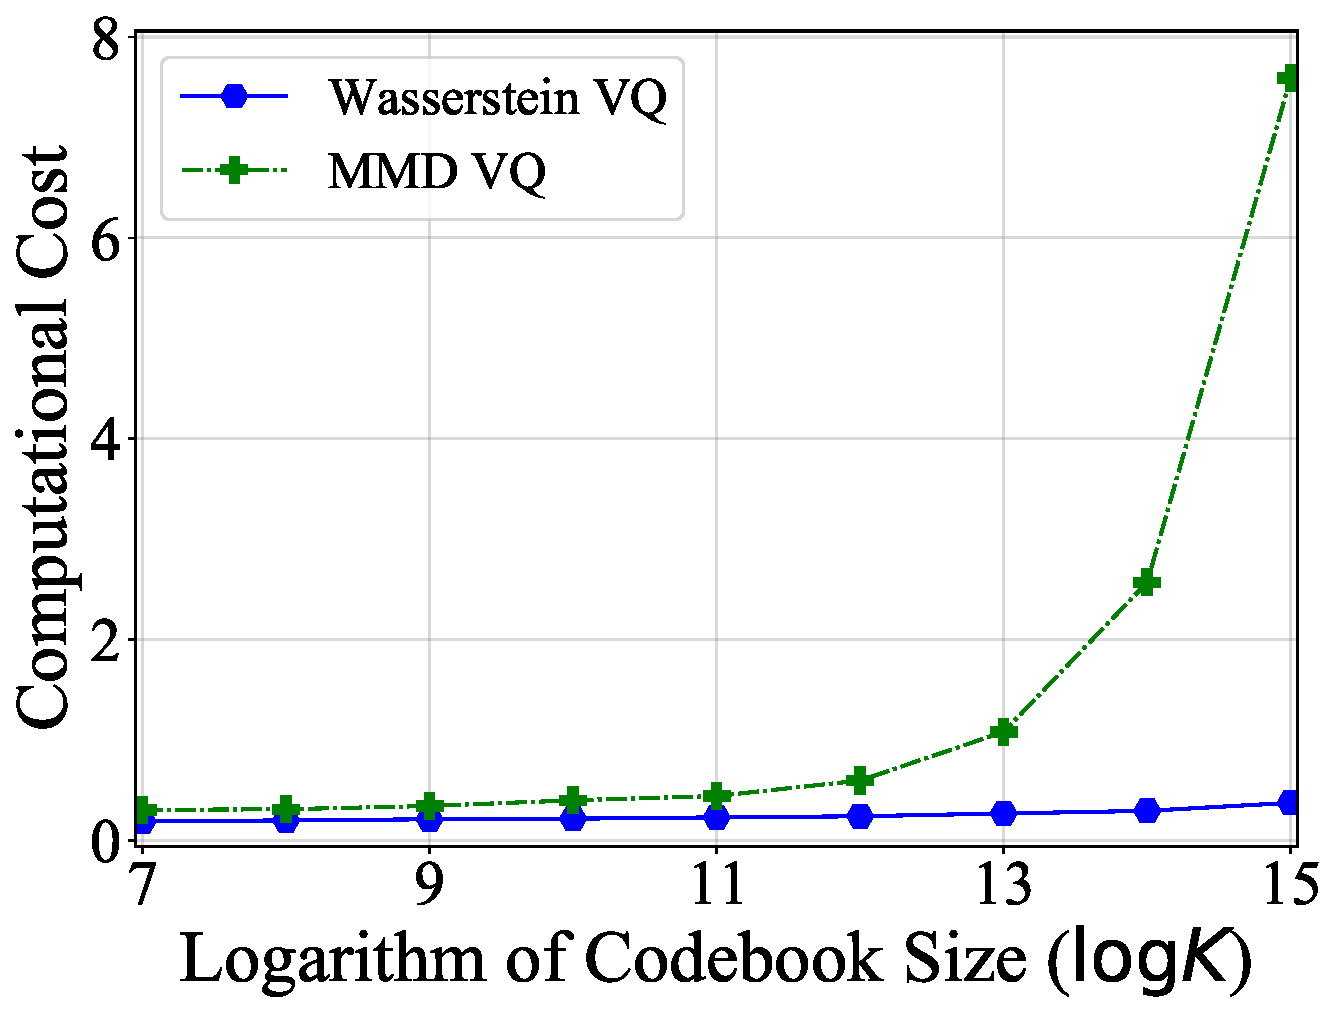
\includegraphics[width=0.475\textwidth]{figs/computational_cost/Computational_Cost_Codebooksize.pdf}
        }
	\subfloat[Data Sample Size]{
		\label{fig:computational-data}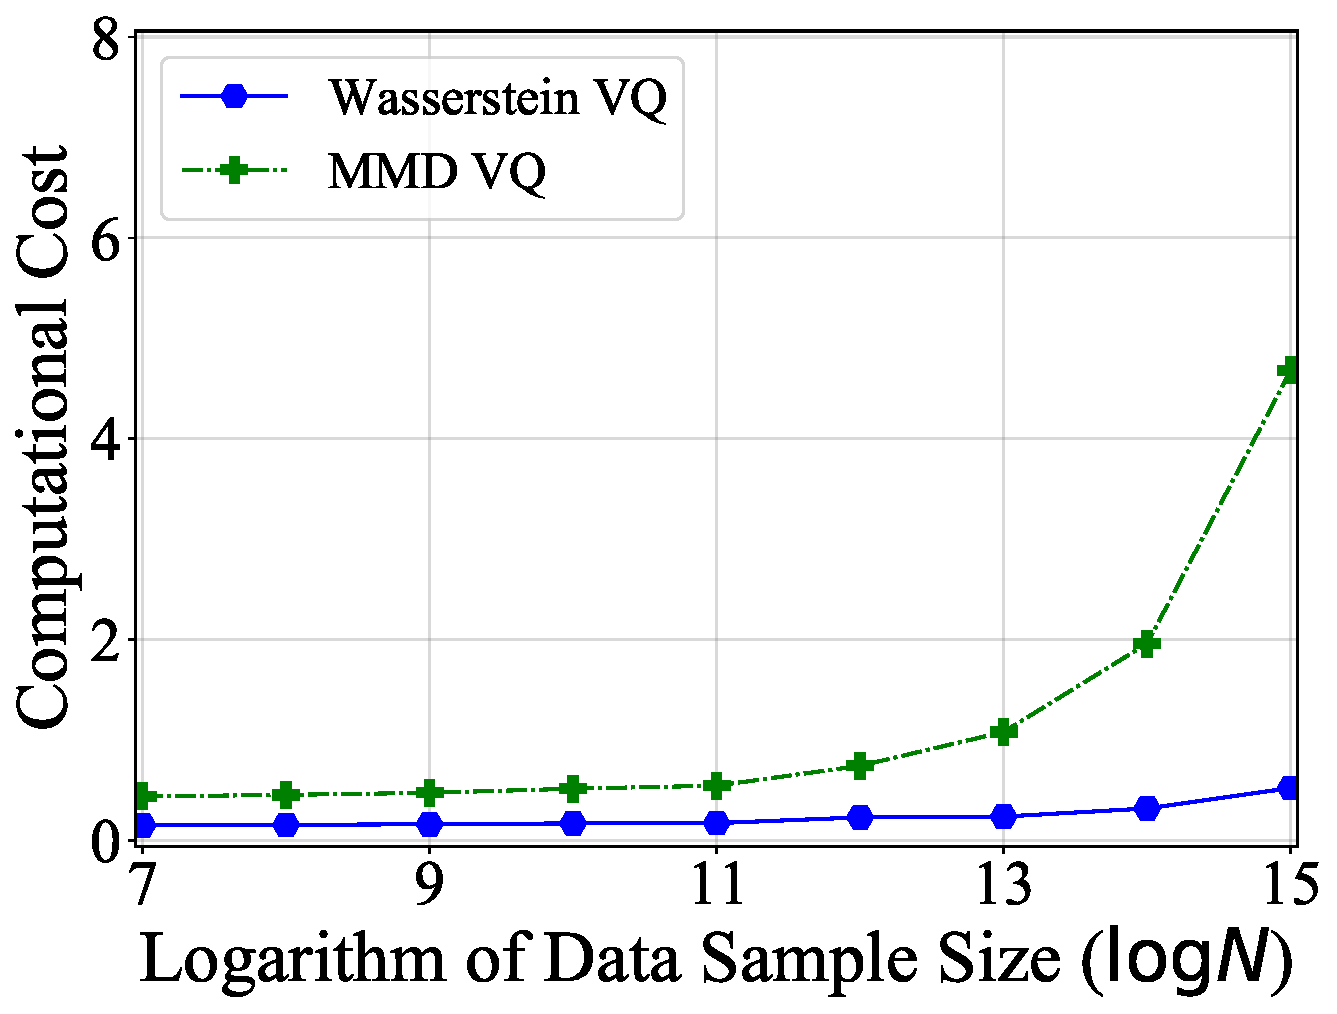
\includegraphics[width=0.475\textwidth]{figs/computational_cost/Computational_Cost_Datasize.pdf}
	}
    \vspace{-2mm}
	\caption{Computational overhead (seconds) comparison between Wasserstein VQ and MMD VQ.}
	\label{fig:computational cost comparison}
    \vspace{-2mm}
\end{figure}

Third, we evaluate the robustness of Wasserstein VQ and MMD VQ under non-Gaussian latent distributions. While Section~\ref{sec:vqvae experiments} shows that the latent distributions in visual tokenization tasks are approximately Gaussian, this experiment allows us to explicitly assess robustness beyond the Gaussian regime. To simulate a non-Gaussian distribution, we follow the setting in Section~\ref{sec:atomic setting} and assume the encoder output features follow a bimodal mixture:
\begin{equation}  
z_i \sim 0.5 \cdot \mathcal{N}(\zeta \mathbf{1}, I) + 0.5 \cdot \mathcal{N}(-\zeta  \mathbf{1}, I), \nonumber
\end{equation}
where the mode separation parameter $\zeta \in \{0.0, 0.5, \dots, 4.0\}$ controls deviation from Gaussianity, with larger $\zeta$ indicating stronger non-Gaussianity. The codebook is initialized with a standard Gaussian distribution, and code vectors are treated as trainable parameters. After 10,000 training steps, we evaluate Wasserstein VQ and MMD VQ in terms of quantization error and codebook utilization rate. As shown in Figures~\ref{fig:comparison quantization error} and~\ref{fig:comparison codebook utilization}, for small $\zeta$ (nearly Gaussian), the two methods perform comparably. As $\zeta$ increases, MMD VQ consistently achieves lower quantization error and higher codebook utilization, whereas Wasserstein VQ degrades due to its limited moment-matching assumption. These synthetic experiments empirically demonstrate that MMD VQ is more robust to non-Gaussian feature distributions.

\paragraph{Summary.}  
Wasserstein VQ and MMD VQ exhibit complementary strengths and limitations. Wasserstein VQ is computationally efficient and performs stably under nearly Gaussian latent distributions, benefiting from its first- and second-order moment-matching formulation, which scales well with large datasets and codebooks. However, it is less robust when feature distributions deviate from Gaussianity. In contrast, MMD VQ excels under non-Gaussian distributions, consistently achieving lower quantization error and higher codebook utilization, but at the cost of substantially higher computational overhead. In practice, Wasserstein VQ is preferred for efficiency and standard Gaussian-like scenarios, while MMD VQ provides an advantage when robustness to non-Gaussian features is critical.
\begin{figure}[!t]
	\centering
    \vspace{-4mm}
    \subfloat[Quantization error]{
		\label{fig:comparison quantization error}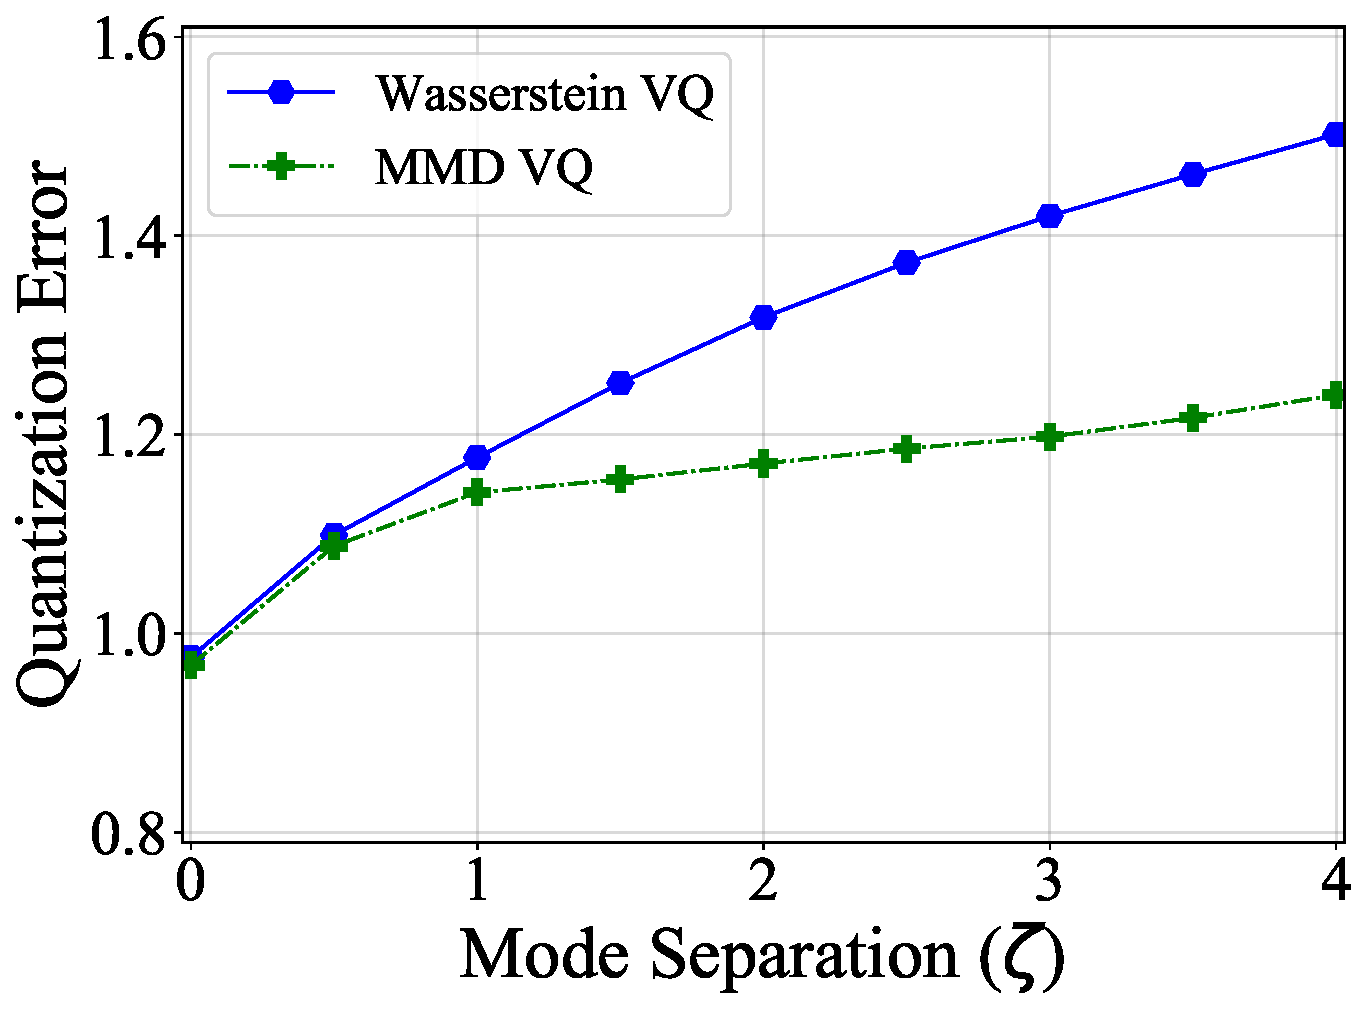
\includegraphics[width=0.475\textwidth]{figs/computational_cost/Quantization_error_Zeta.pdf}
	}
	\subfloat[Codebook utilization]{ 
		\label{fig:comparison codebook utilization}  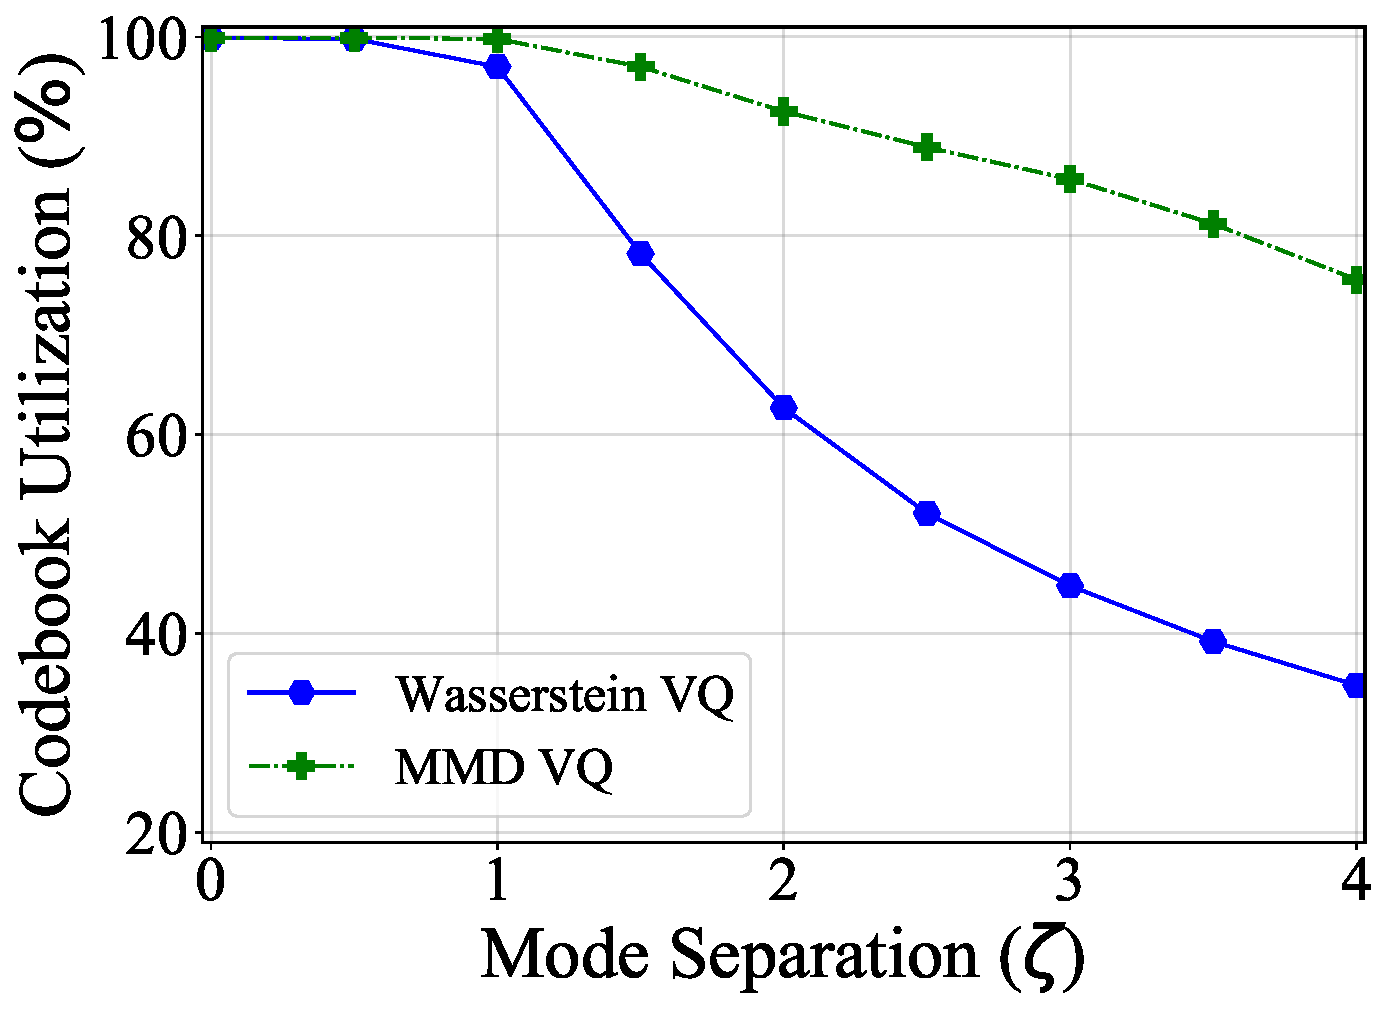
\includegraphics[width=0.475\textwidth]{figs/computational_cost/CodebookUtilization_Zeta.pdf}
        }
    \vspace{-1mm}
	\caption{ comparison between Wasserstein VQ and MMD VQ.}
	\label{fig:comparison non-gaussian}
    \vspace{-5mm}
\end{figure}